\section{PRIMER TEMA}
	\subsection{Aisladores Sísmicos}
Son dispositivos que desacoplan la estructura y su contenido de los efectos de un sismo. Este desacople se alcanza incrementando la flexibilidad del sistema y proporcionándole un amortiguamiento adecuado \shortcites{Skinner1993}\citep{Skinner1993}.

Existen diversos tipos de aisladores sísmicos, siendo los más usados en la actualidad los aisladores elastoméricos y los aisladores friccionantes.

		\subsubsection{Aisladores Elastoméricos}
\begin{itemize}

\item Aisladores de elastómero natural o de bajo amortiguamiento

Los dispositivos NRB (\textit{Natural Rubber Bearing}) consisten en capas alternadas de caucho y acero unidas mediante un proceso de vulcanización. Se caracterizan por su bajo nivel de amortiguamiento (alrededor de 2-3\%), poseen una curva fuerza deformación casi lineal y una fuerza restitutiva estable \citep{Kelly1999}.

\end{itemize}

		\subsubsection{Aisladores Friccionantes}
\begin{itemize}

\item Aisladores de péndulo de fricción simple

Los dispositivos FPS (\textit{Frictional Pendulum System}) constan de un deslizador articulado que se mueve sobre una superficie de fricción esférica. La superficie de contacto está revestida de un material compuesto autolubricante. Cuando el deslizador se mueve sobre la superficie esférica, la masa soportada se levantará y el movimiento proporcionará la fuerza restitutiva del sistema. El radio de curvatura de la superficie cóncava dominará la rigidez y el periodo del sistema \citep{Wu2001}.

\end{itemize}


	\begin{figure}[!h]
	\centering
	\begin{subfigure}[b]{0.45\textwidth}
  	\centering
  	% include first image
  	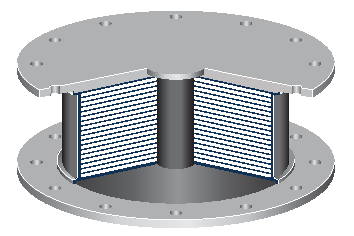
\includegraphics[scale=1]{E_IMAGENES/1_Capitulo2/Cap2_Imagen1a.pdf}
	\caption{\centering\footnotesize Aislador eslastomérico LRB. Adaptado de \citet{Bridgestone2015}}
  	\label{Cap2_Figura1a}
	\end{subfigure}
	\hfill
	\begin{subfigure}[b]{0.45\textwidth}
  	\centering
  	% include second image
  	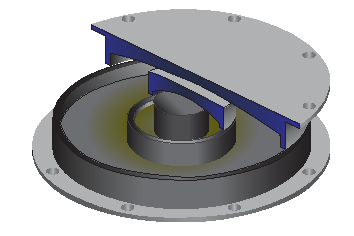
\includegraphics[scale=1]{E_IMAGENES/1_Capitulo2/Cap2_Imagen1b.pdf} 
  	\caption{\centering\footnotesize Aislador friccionante TFPB. Adaptado de \citet{Fenz2008}}
  	\label{Cap2_Figura1b}
	\end{subfigure}
	\caption[Dispositivos de aislamiento sísmico]{\centering\footnotesize Dispositivos de aislamiento sísmico}
	\label{Cap2_Figura1}
	\end{figure}
	
	\subsection{Disipadores de Fluido Viscoso}
Son dispositivos que incrementan el amortiguamiento de la estructura sin incrementar la rigidez y cuyo funcionamiento depende fundamentalmente de la velocidad relativa de sus extremos. Los DFV están compuestos por un pistón de acero inoxidable, con cabezal de bronce y un acumulador, que se encuentran alojados dentro en un cilindro metálico lleno con un fluido de alta viscosidad. La cabeza del pistón tiene orificios que están diseñados con una serie de formas especiales para alterar las características de flujo con la velocidad del fluido, disipando de esta manera energía en forma de calor. La construcción mecánica y las propiedades del orificio se pueden variar para obtener las propiedades amortiguadoras deseadas \citep{Constantinou1993}.

	\begin{figure}[!h]
	\centering
		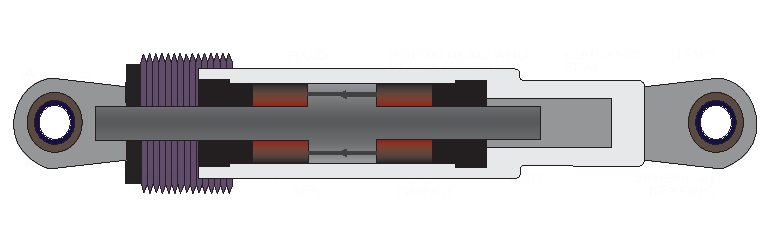
\includegraphics[scale=1]{E_IMAGENES/1_Capitulo2/Cap2_Imagen2.pdf}
	\caption[Disipador de fluido viscoso]{\centering\footnotesize Disipador de fluido viscoso.  Adaptado de \shortcites{Taylor2019}\citet{Taylor2019}}
	\label{Cap2_Figura2}
	\end{figure}
	
	
	
	
